\renewcommand{\thefootnote}{\fnsymbol{footnote}}

\chapter[First theorem of welfare economics]%
 {First theorem of welfare economics}%
\label{ch:L8}

% 3) Reset things so later footnotes go back to 1, 2, 3, …
%\setcounter{footnote}{0}
\renewcommand{\thefootnote}{\arabic{footnote}}

%\section{A preliminary lemma}\label{sec:L8-intro}

We start with a preliminary lemma. All the proofs here are by contradiction. The logic of these proofs is as follows. We want to prove some statement \( S \). We assume that \( S \) is false, and we show that this assumption leads to a contradiction, that is, some conclusion of the type \( C \) and \textbf{not} \( C \), which is impossible. Therefore, \( S \) must be true.

\begin{lemma}\label{lem:lns}
    Assume preferences \( \succsim_i \) are locally non-satiated. Let \( x_i \in D_i (p,e_i) \). If \( x'_i \succsim_i x_i \), then \( p \cdot x'_i \ge p \cdot x_i \).
\end{lemma}

\begin{proof}
    Suppose not. Then \( p \cdot x'_i < p \cdot x_i \). By local non-satiation, there exists \( x''_i \) such that \( \|x''_i - x'_i\| < \varepsilon \) and \( x''_i \succ_i x'_i \). By choosing \( \varepsilon \) small enough, we can ensure that \( p \cdot x''_i < p \cdot x_i \). But then \( x''_i \in B(e_i,p) \) and \( x''_i \succ_i x_i \), by transitivity, contradicting the fact that \( x_i \in D_i (e_i, p) \).
\end{proof}

%\subsection{The main result}

\begin{theorem}\label{thm:fftwe} (\textbf{First fundamental theorem of welfare economics}) If preferences in the economy \( E \) are locally non-satiated, then every allocation selected by a Walrasian equilibrium with transfers is Pareto optimal. That is,

    \[
        x \in R^{WT} (E) \quad \Longrightarrow \quad x \quad \text{is Pareto optimal}.
    \]
\end{theorem}

\begin{proof}
    Let \(E\) be an economy and suppose that \(x \in R^{WT}(E)\).
    Then there exist strictly positive prices \(p\) and transfers
    \((T_i)_{i\in I}\) such that, for every individual \(i\),
    \[
        x_i \in D_i(e_i + T_i,p),
    \]
    that is, \(x_i\) is a most preferred bundle in the budget set
    \(B(e_i+T_i,p)\).

    Suppose, towards a contradiction, that \(x\) is not Pareto optimal.
    Then there exists a feasible allocation \(x'\) such that
    \(x'_i \succsim_i x_i\) for all \(i\), and
    \(x'_j \succ_j x_j\) for some individual \(j\).
    By the Lemma \ref{lem:lns}, local non-satiation implies
    \[
        p\cdot x'_i \ge p\cdot x_i \quad \forall i,
        \qquad
        p\cdot x'_j > p\cdot x_j.
    \]
    Summing over all individuals,
    \[
        \sum_{i\in I} p\cdot x'_i > \sum_{i\in I} p\cdot x_i.
    \]

    On the other hand, feasibility of \(x'\) implies
    \[
        \sum_{i\in I} x'_i \le \sum_{i\in I} e_i
        = \sum_{i\in I} x_i,
    \]
    since \(x\) is feasible as well.
    Multiplying the inequality
    \(\sum_i (x'_i - x_i) \le 0\)
    by the strictly positive price vector \(p\) yields
    \[
        \sum_{i\in I} p\cdot x'_i
        \le \sum_{i\in I} p\cdot x_i,
    \]
    contradicting the strict inequality obtained above.
    Hence no such \(x'\) exists, and
    \(x\) is Pareto optimal.
\end{proof}

Let us discuss why Local non-satiation is necessary for Theorem \ref{thm:fftwe} to hold. Individual \( 1 \) has \textquote{thick} indifference curves, thus violating local non-satiation. The allocation \( x \) is not Pareto optimal, since we can find another feasible allocation \( x' \) that makes individual \( 2 \) strictly better off without making individual \( 1 \) worse off. However, \( x \) can still be supported as a Walrasian equilibrium with transfers at prices \( p \). Thus, without local non-satiation, Theorem \ref{thm:fftwe} fails.

\begin{figure}[H]
    \begin{center}
        \tikzset{every picture/.style={line width=0.75pt}} %set default line width to 0.75pt        

        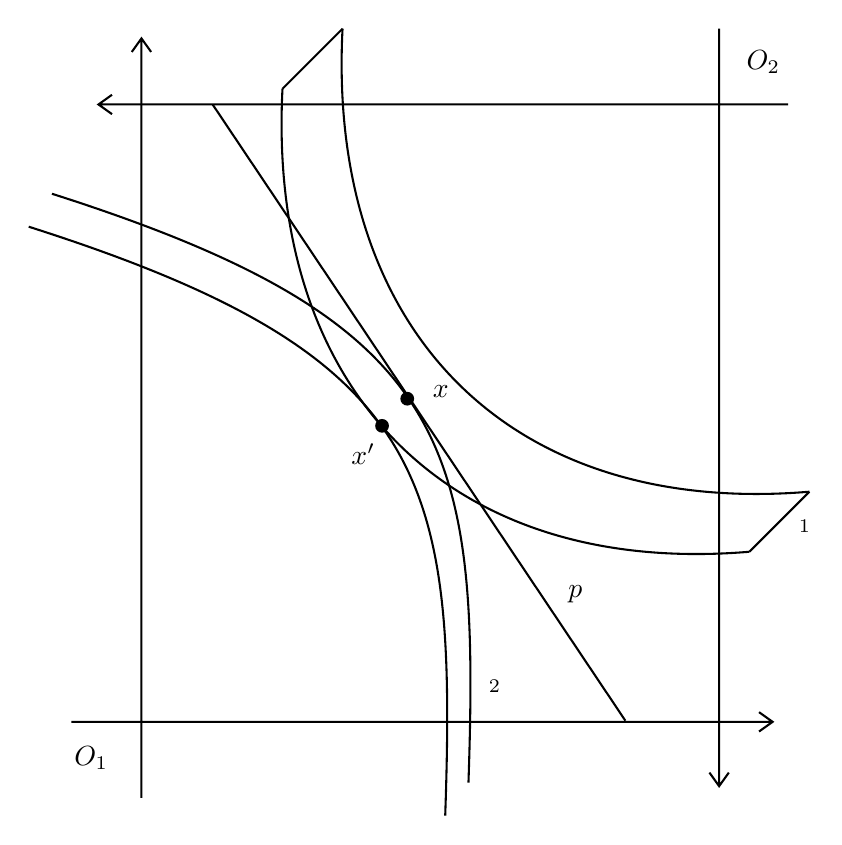
\begin{tikzpicture}[x=0.70pt,y=0.70pt,yscale=-1,xscale=1]
            %uncomment if require: \path (0,443); %set diagram left start at 0, and has height of 443

            %Shape: Axis 2D [id:dp22115699468612893] 
            \draw  (140,370.4) -- (502,370.4)(176.2,17.6) -- (176.2,409.6) (495,365.4) -- (502,370.4) -- (495,375.4) (171.2,24.6) -- (176.2,17.6) -- (181.2,24.6)  ;
            %Shape: Axis 2D [id:dp32207533916759135] 
            \draw  (510,51.7) -- (154,51.7)(474.4,403.6) -- (474.4,12.6) (161,56.7) -- (154,51.7) -- (161,46.7) (479.4,396.6) -- (474.4,403.6) -- (469.4,396.6)  ;
            %Curve Lines [id:da8559403196511832] 
            \draw    (249,43.6) .. controls (241,199.6) and (335,295.6) .. (490,282.6) ;
            %Curve Lines [id:da37662840950707166] 
            \draw    (280,12.6) .. controls (272,168.6) and (366,264.6) .. (521,251.6) ;
            %Straight Lines [id:da5642668535456735] 
            \draw    (249,43.6) -- (280,12.6) ;
            %Straight Lines [id:da9097139754709688] 
            \draw    (490,282.6) -- (521,251.6) ;
            %Curve Lines [id:da09819389723996741] 
            \draw    (130,97.8) .. controls (337,163.8) and (351,225.8) .. (345,401.8) ;
            %Shape: Circle [id:dp16582666368555876] 
            \draw  [fill={rgb, 255:red, 0; green, 0; blue, 0 }  ,fill opacity=1 ] (310.4,203.6) .. controls (310.4,201.94) and (311.74,200.6) .. (313.4,200.6) .. controls (315.06,200.6) and (316.4,201.94) .. (316.4,203.6) .. controls (316.4,205.26) and (315.06,206.6) .. (313.4,206.6) .. controls (311.74,206.6) and (310.4,205.26) .. (310.4,203.6) -- cycle ;
            %Shape: Circle [id:dp20605667579120546] 
            \draw  [fill={rgb, 255:red, 0; green, 0; blue, 0 }  ,fill opacity=1 ] (297.4,217.6) .. controls (297.4,215.94) and (298.74,214.6) .. (300.4,214.6) .. controls (302.06,214.6) and (303.4,215.94) .. (303.4,217.6) .. controls (303.4,219.26) and (302.06,220.6) .. (300.4,220.6) .. controls (298.74,220.6) and (297.4,219.26) .. (297.4,217.6) -- cycle ;
            %Curve Lines [id:da6954752398238686] 
            \draw    (118,114.8) .. controls (325,180.8) and (339,242.8) .. (333,418.8) ;
            %Straight Lines [id:da49767621503014337] 
            \draw    (213,51.8) -- (426,369.8) ;

            % Text Node
            \draw (140,381.4) node [anchor=north west][inner sep=0.75pt]    {$O_{1}$};
            % Text Node
            \draw (487,22.4) node [anchor=north west][inner sep=0.75pt]    {$O_{2}$};
            % Text Node
            \draw (514,264.4) node [anchor=north west][inner sep=0.75pt]    {$\succsim _{1}$};
            % Text Node
            \draw (325,195.4) node [anchor=north west][inner sep=0.75pt]    {$x$};
            % Text Node
            \draw (283,225.4) node [anchor=north west][inner sep=0.75pt]    {$x'$};
            % Text Node
            \draw (354,347.4) node [anchor=north west][inner sep=0.75pt]    {$\succsim _{2}$};
            % Text Node
            \draw (395,298.4) node [anchor=north west][inner sep=0.75pt]    {$p$};
        \end{tikzpicture}
        \label{fig:lns-fwelf}
        \caption{Local Non-Satiation is necessary for the First Welfare Theorem.}
    \end{center}
\end{figure}

Let us now interpret Theorem \ref{thm:fftwe}. A standard question in economics is how to allocate resources given data on preferences.\footnote{In the most general form, a question of this kind is asked in \cite{arrowSocialChoiceIndividual2012}.} We might want such an allocation of resources to satisfy some good properties from a \textit{normative} perspective. One such property is Pareto optimality. An allocation rule taking preferences and endowments as inputs and returning a Pareto optimal allocation as output might therefore be desirable. However, once one has an allocation rule, one might wonder whether such an allocation rule could be implemented in a decentralized way. A rule taking preferences and endowments as inputs and returning allocations as output does not tell us \textit{how} to reach such allocations. Theorem \ref{thm:fftwe} tells us that the Walrasian equilibrium with transfers implements an allocation rule always delivering Pareto optimal allocations. There is a bit more, however. A Walrasian equilibrium with transfers is not just a mechanism to implement Pareto optimal allocations. It delivers prices for each good allowing to trade so to reach such allocations. Prices may be interpreted as \textquote{values} for goods, where these values depends on the preferences all individuals in the economy. In fact, \cite{debreuTheoryValueAxiomatic1959} is titled \textit{Theory of Value:}. A lot of more or less sophisticated critiques of economics stem from the idea that it is inappropriate to view the value of goods as determined by prices. In fact, there is famous citation, misattributed to Oscar Wilde,\footnote{Apparently the original citation is.} that says: \textquote{An economist is someone who knows the price of everything and the value of nothing}. Of course, there are legitimate reason to question weather values should be entirely derived from individual preferences. But there is nothing special in prices that is not related to preferences, in the setting under consideration here.

Unfortunately, an allocation rule delivering Pareto optimal allocations can sometimes be undesirable from other points of view. For instance, such an allocation rule might deliver very unequal allocations. Let us consider a second property we might want an allocation to satisfy.

\begin{definition}
    An allocation \( x \) is \textbf{envy-free} if for all individuals \( i, j \), \( x_i \succsim_i x_j \).
\end{definition}

An allocation is envy-free if no individual prefers someone else's bundle to her own. Envy-freeness is a desirable property from a fairness perspective.\footnote{For recent and deeper analyses of envy-freeness, check \cite{fleurbaeyFairnessResponsibilityWelfare2008} and \cite{thomsonFairAllocationRules2011}.} In particular, envy-freeness is strongly related to the idea of equality of opportunity. A way of looking at such relationship is captured in the following proposition.

\begin{proposition}\label{prop:envy}
    Every allocation selected by an Egalitarian Walrasian equilibrium is envy-free. That is,
    \[
        x \in R^{EW}(E) \quad \Longrightarrow \quad x \quad \text{is envy-free}.
    \]
\end{proposition}

\begin{proof}
    Let \( E \) be an economy and suppose that \( x \in R^{EW}(E) \). By definition of the Egalitarian Walrasian rule, there exists a price vector \( p \in \mathbb{R}^\ell_{++} \) such that, for every individual \( i \in I \),
    \[
        x_i \in D_i\!\left(\frac{\bar e}{n},p\right),
    \]
    where \( D_i(e,p) \) denotes the set of most preferred bundles of \( i \) in the budget set
    \[
        B(e,p) = \{\, x' \in \mathbb{R}^\ell_+ \mid p \cdot x' \le p \cdot e \,\}.
    \]

    Because all individuals face the same ``egalitarian'' endowment \( \frac{\bar e}{n} \) and the same price vector \( p \), they all face the same budget set
    \[
        B := B\!\left(\frac{\bar e}{n},p\right)
        = \{\, x' \in \mathbb{R}^\ell_+ \mid p \cdot x' \le p \cdot \tfrac{\bar e}{n} \,\}.
    \]

    Fix any individual \( i \). Since \( x_i \in D_i\!\left(\frac{\bar e}{n},p\right) \), \( x_i \) is a most preferred bundle for \( i \) in \( B \). Therefore,
    \begin{equation}
        \label{eq:maximal}
        \forall x' \in B,\qquad x_i \succsim_i y.
    \end{equation}

    Now consider any other individual \( j \in I \). Because \( x_j \in D_j\!\left(\frac{\bar e}{n},p\right) \), we also have \( x_j \in B \). Applying \eqref{eq:maximal} to the specific bundle \( x' = x_j \) yields
    \[
        x_i \succsim_i x_j.
    \]

    Thus, for every pair of individuals \( i,j \in I \), consumer \( i \) (weakly) prefers her own allocation \( x_i \) to the allocation \( x_j \) of consumer \( j \):
    \[
        \forall i,j \in I,\qquad x_i \succsim_i x_j.
    \]

    In particular, this implies that there is no pair \( i \neq j \) for which \( x_j \succ_i x_i \). Hence no individual strictly prefers someone else's bundle to her own.

    Therefore, the allocation \( x \) is envy-free.
\end{proof}

By Theorem \ref{thm:fftwe} and Proposition \ref{prop:envy}, we know that the Walrasian Egalitarian allocation rule delivers allocations that are both Pareto optimal and envy-free. However, endowments might be distinct from the egalitarian endowment \( \frac{\bar e}{n} \). We might therefore be interested in knowing how to implement such allocation rule. The Second Fundamental Theorem of Welfare Economics, which we will discuss in the next chapter, provides conditions under which this is possible.

\paragraph{Things to read.} This lecture is based on \citet[pp. 545-550]{mas-colellMicroeconomicTheory1995}.

\section{Exercises}

hey.

\bibliographystyle{apacite}  % or another  style
\bibliography{references} % .bib file goes in ./bib/